\chapter{Diagrammes de blocs de définition}
\section{Diagramme de blocs général}
Afin de répondre à l'ensemble des exigences présentées section \ref{req}, figure \ref{fig:requirements}, la salle de bain possède différents blocks : 
\begin{description}
	\item[Mobilier] Concerne les équipements devant s'adapter à l'habitant
	\item[Eclairage] Tout ce qui est prévu pour l'adaptation de l'éclairage 
	\item[Radiateurs] L'adaptation de la température de la pièce
	\item[Contrôleur] Un système permettant de contrôler les éléments de notre salle de bain. Ce système contient un micro-contrôleur permettant l'utilisation des capteurs et actionneurs, un système de
		communication avec les données de la maison intelligente, ainsi qu'un logiciel effectuant les traitements nécessaires (monter/descendre un mobilier, augmenter la température de la pièce,
		\ldots)
\end{description}

\begin{figure}[H]
	\centering
	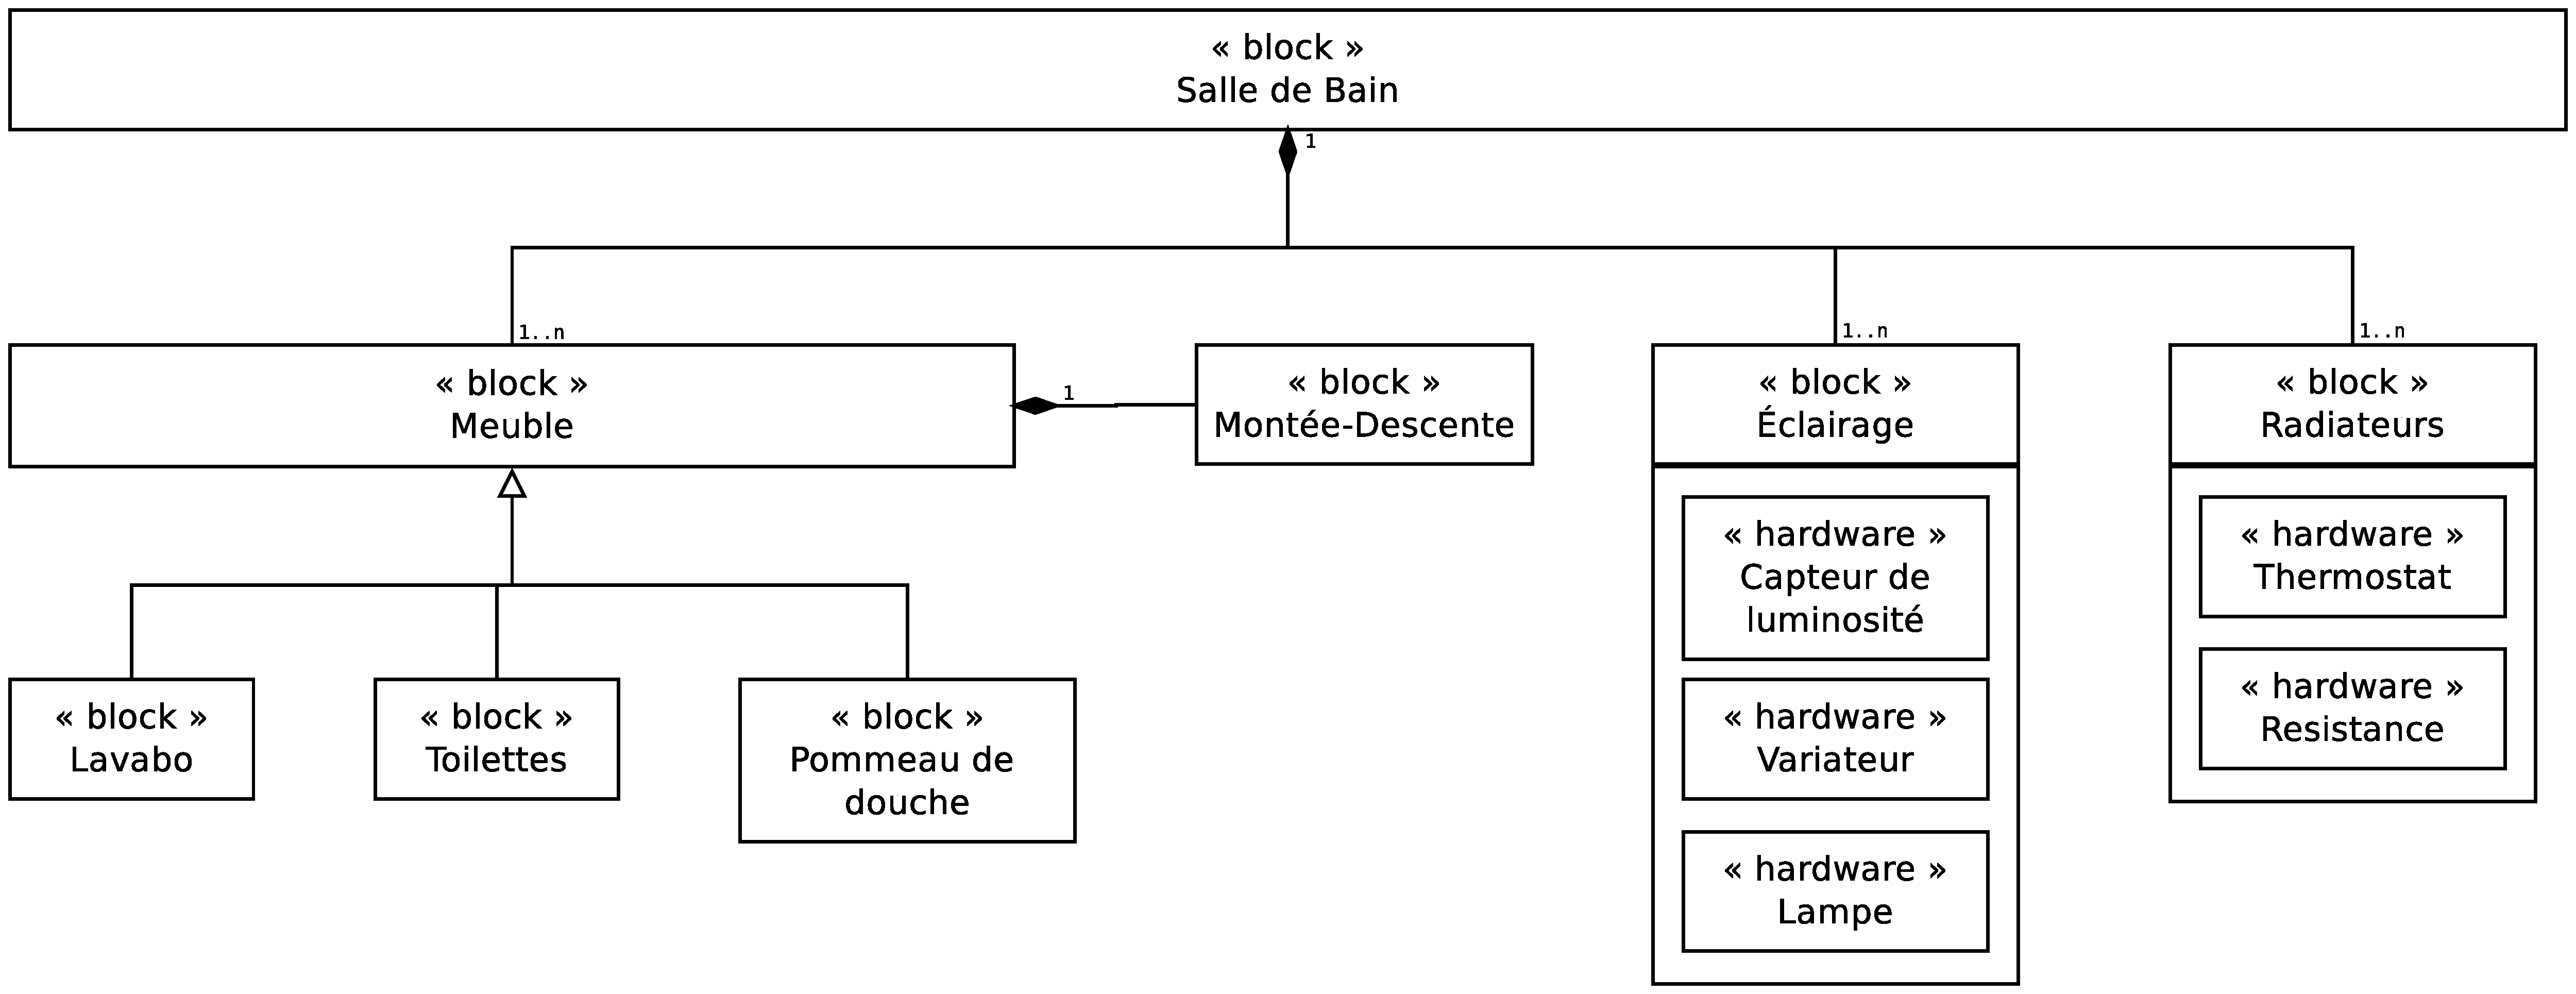
\includegraphics[width=1\linewidth]{diagrams/bathroom/diagramme_blocks_bdd.eps}
	\caption{Diagramme de bloc de définition}
	\label{fig:diagramme_bdd}
\end{figure}

\section{Diagramme de bloc de « Montée-Descente »}
Chaque mobilier doit pouvoir moduler sa hauteur pour s'adapter à l'habitant de la MI. Chaque mobilier de la salle de bain est doté d'un bloc « Montée-Descente » comportant :
\begin{description}
	\item[Capteur de mouvement Infra-Rouge] détermine les mouvements de l'habitant
	\item[Capteur laser] permet de déterminer la taille de l'habitant afin de pouvoir s'adapter à lui
	\item[Système élévateur] permet de monter ou descendre la dalle supportant le mobilier (ou l'habitant si celui-ci est dans la douche) en fonction de sa position actuelle et de la taille de l'habitant.   
\end{description}

\begin{figure}[H]
	\centering
	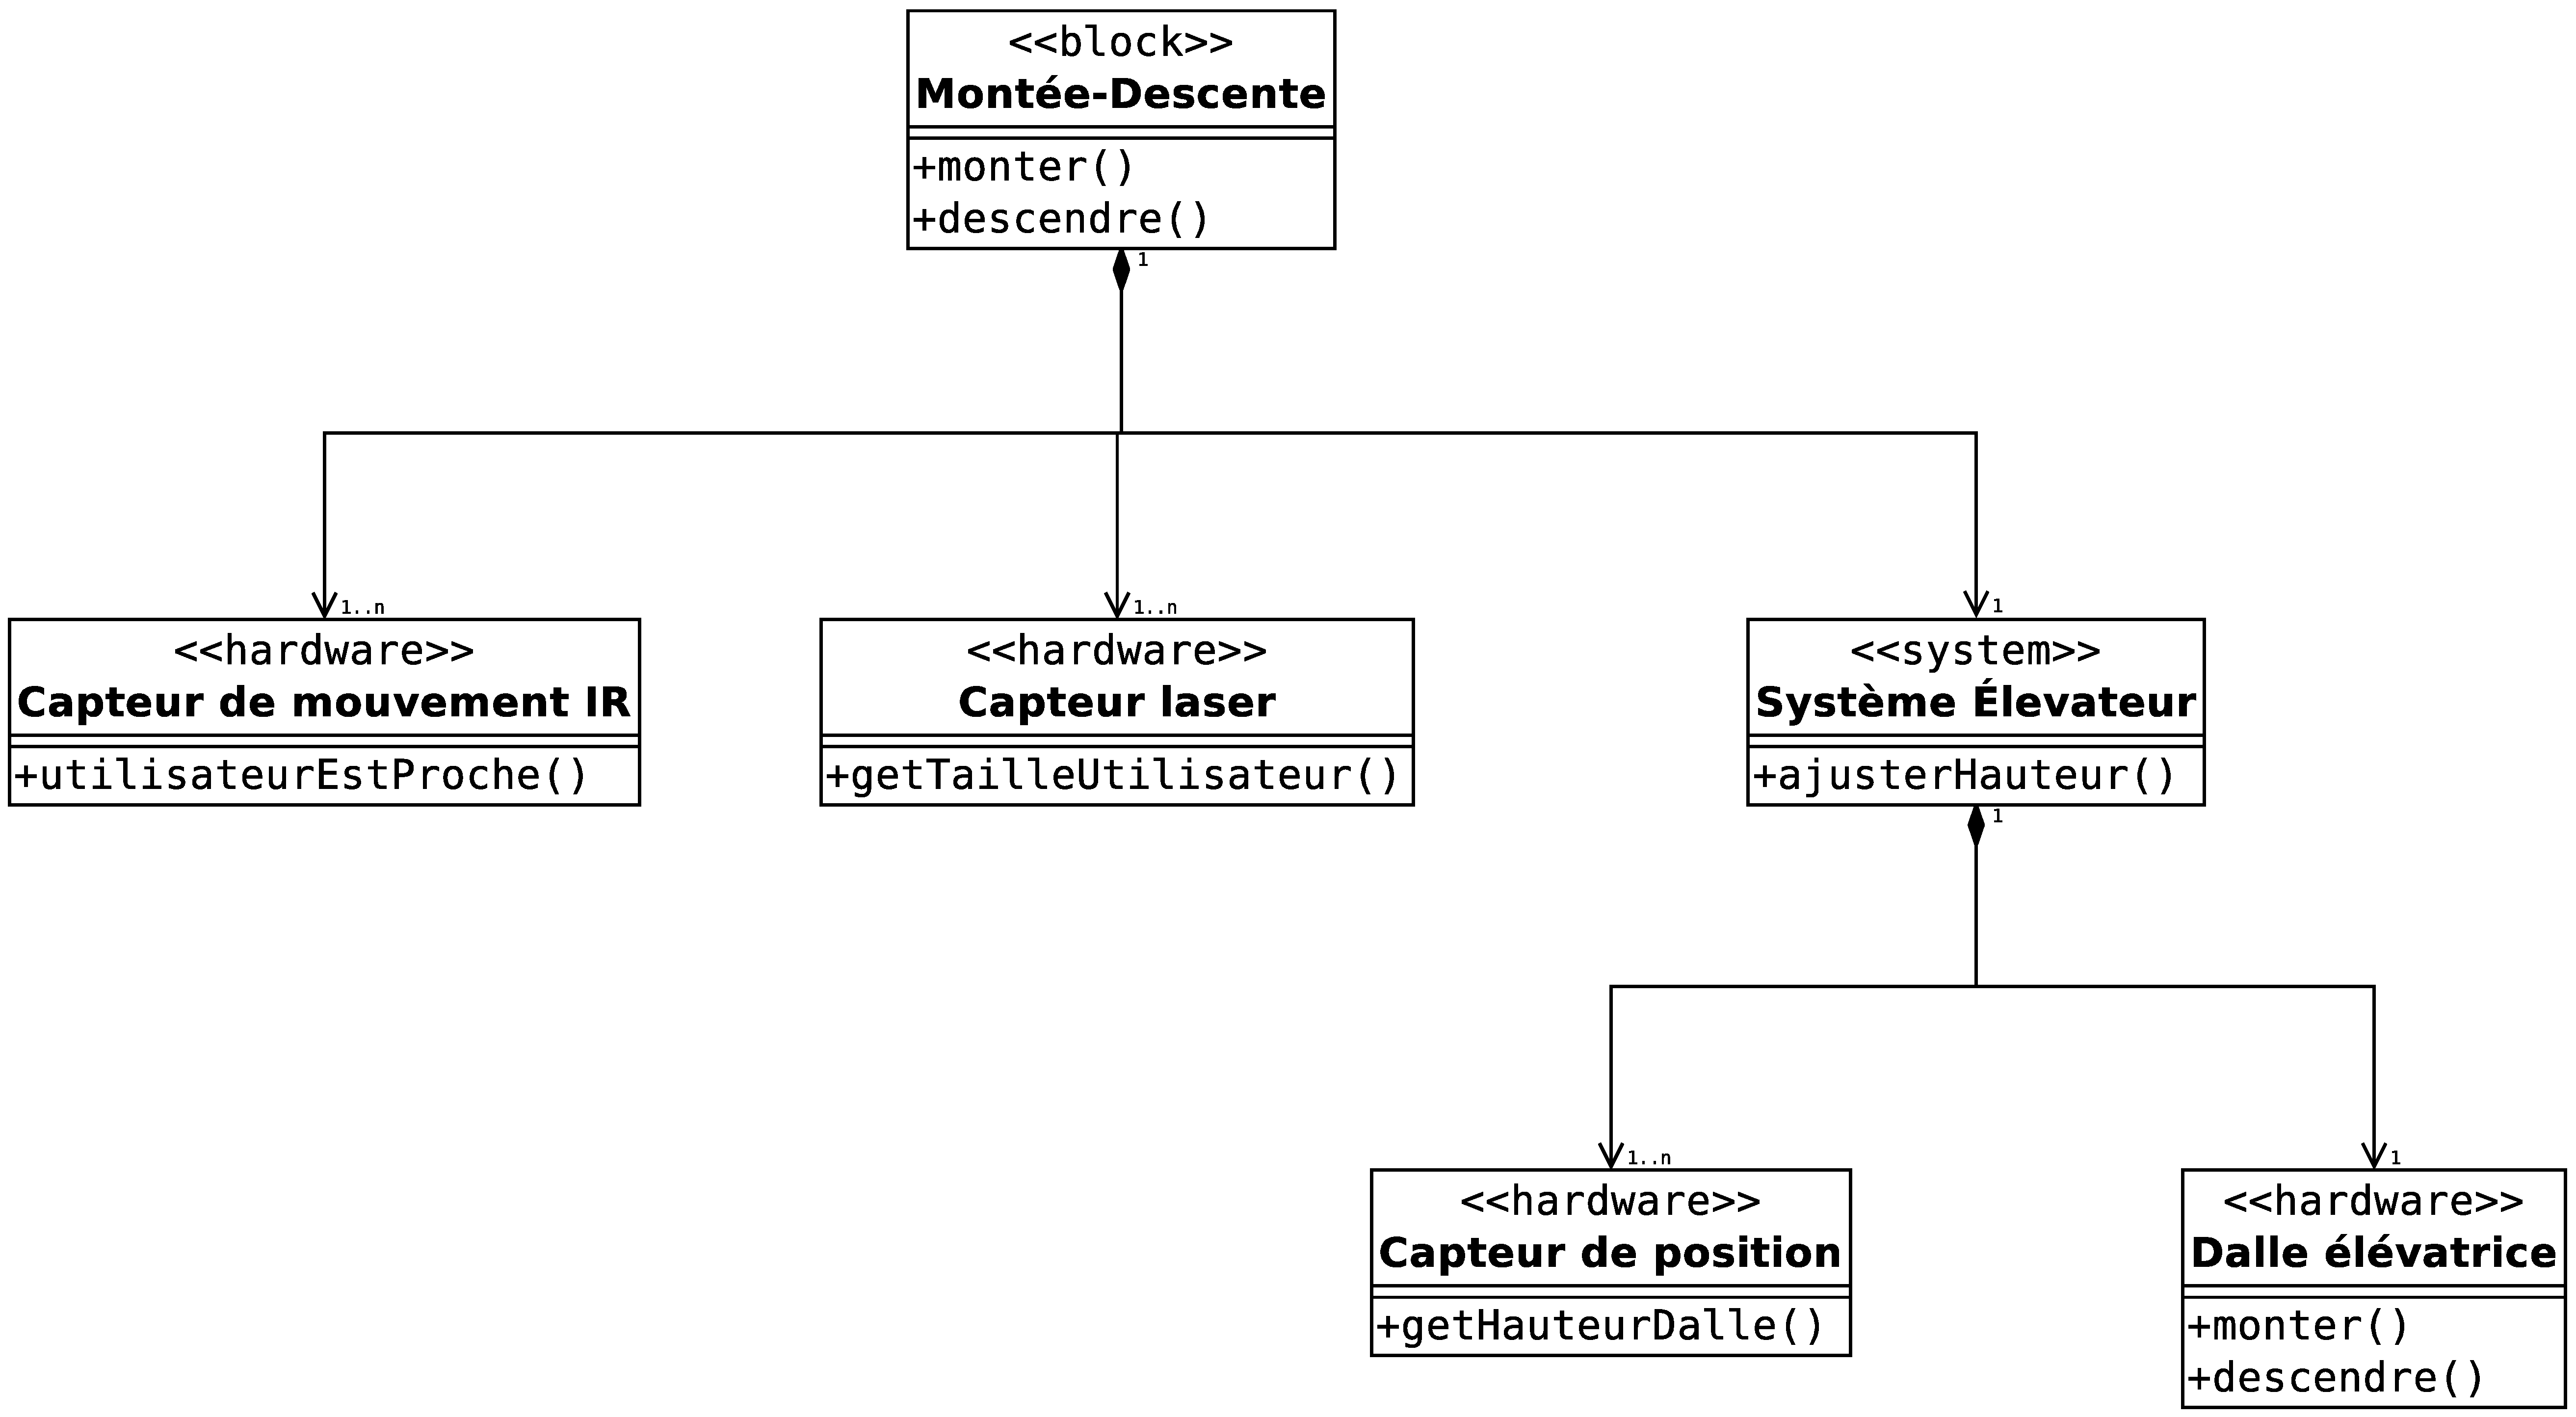
\includegraphics[width=1\linewidth]{diagrams/bathroom/diagramme_blocks_bdd2.eps}
	\caption{Diagramme de bloc de définition de « Montée-Descente »}
	\label{fig:diagramme_bdd2}
\end{figure}
